\documentclass{beamer}

% Theme and color scheme
\usetheme{Madrid}
\usecolortheme{default}

% Packages
\usepackage{graphicx}
\usepackage{amsmath}
\usepackage{amssymb}
\usepackage{booktabs}
\usepackage{tikz}
\usepackage{algorithm}
\usepackage{algpseudocode}
\usepackage{hyperref}

% Title information
\title[Multimodal Depression Detection]{Multimodal Depression Detection System for Dravidian Languages}
\subtitle{22AIE315 Natural Language Processing - Term Project}

\author[Team A15]{
Team A15\\[0.4em]
Keerthivasan SV (CB.SC.U4AIE23037)\\
Krish S (CB.SC.U4AIE23040)\\
Sriranjana (CB.SC.U4AIE23066)\\
Thrishala (CB.SC.U4AIE23072)
}

\date{January 2026}

\begin{document}

% Title Slide
\begin{frame}
\titlepage
\end{frame}

% Project Overview & Course Alignment
\begin{frame}
\frametitle{Project Overview \& Course Alignment}
\begin{itemize}
    \item \textbf{Problem}: Depression detection in low-resource Dravidian languages (Tamil, Malayalam)
    \item \textbf{NLP Course Objectives Addressed}:
    \begin{itemize}
        \item \textbf{CO1}: Modern computational linguistics tools for morphology and syntax analysis
        \item \textbf{CO2}: Word representation models (TF-IDF, neural embeddings, transformers)
        \item \textbf{CO3}: Deep learning models for NLP applications (RNN, LSTM, BERT)
        \item \textbf{CO4}: Comprehensive evaluation metrics and performance analysis
    \end{itemize}
    \item \textbf{Key Achievement}: 95.2\% accuracy using multimodal NLP approach
\end{itemize}
\end{frame}

% NLP Techniques Implemented
\begin{frame}
\frametitle{NLP Techniques Implemented (Syllabus Coverage)}
\begin{itemize}
    \item \textbf{Unit 1 - Computational Linguistics}:
    \begin{itemize}
        \item Morphological analysis for agglutinative Tamil/Malayalam
        \item Syntactic parsing with dependency trees
        \item Semantic analysis for depression markers
    \end{itemize}
    \item \textbf{Unit 2 - Word Representations}:
    \begin{itemize}
        \item TF-IDF vectorization for baseline models
        \item Neural word embeddings (Word2Vec, FastText)
        \item Transformer-based contextualized embeddings (BERT, MuRIL)
    \end{itemize}
    \item \textbf{Unit 3 - Sequential Models}:
    \begin{itemize}
        \item LSTM networks for temporal audio-text modeling
        \item Attention mechanisms for multimodal fusion
        \item BERT fine-tuning for Dravidian language understanding
    \end{itemize}
\end{itemize}
\end{frame}

% Unit 4 Applications - Core NLP Tasks
\begin{frame}
\frametitle{Unit 4 Applications - Core NLP Tasks Implemented}
\begin{itemize}
    \item \textbf{Traditional NLP Pipeline}:
    \begin{itemize}
        \item \textbf{Part-of-Speech Tagging}: Rule-based + statistical for Tamil/Malayalam
        \item \textbf{Named Entity Recognition}: Person, location, organization detection
        \item \textbf{Dependency Parsing}: Syntactic relationship extraction
        \item \textbf{Sentiment Analysis}: Depression-specific sentiment classification
    \end{itemize}
    \item \textbf{Advanced Applications}:
    \begin{itemize}
        \item Text classification for depression detection
        \item Multimodal fusion combining text and audio features
        \item Real-time text processing and analysis
    \end{itemize}
    \item \textbf{Evaluation Metrics}: Precision, Recall, F1-Score, Accuracy, Confusion Matrix
\end{itemize}
\end{frame}

% System Architecture
\begin{frame}
\frametitle{NLP System Architecture}
\begin{center}
    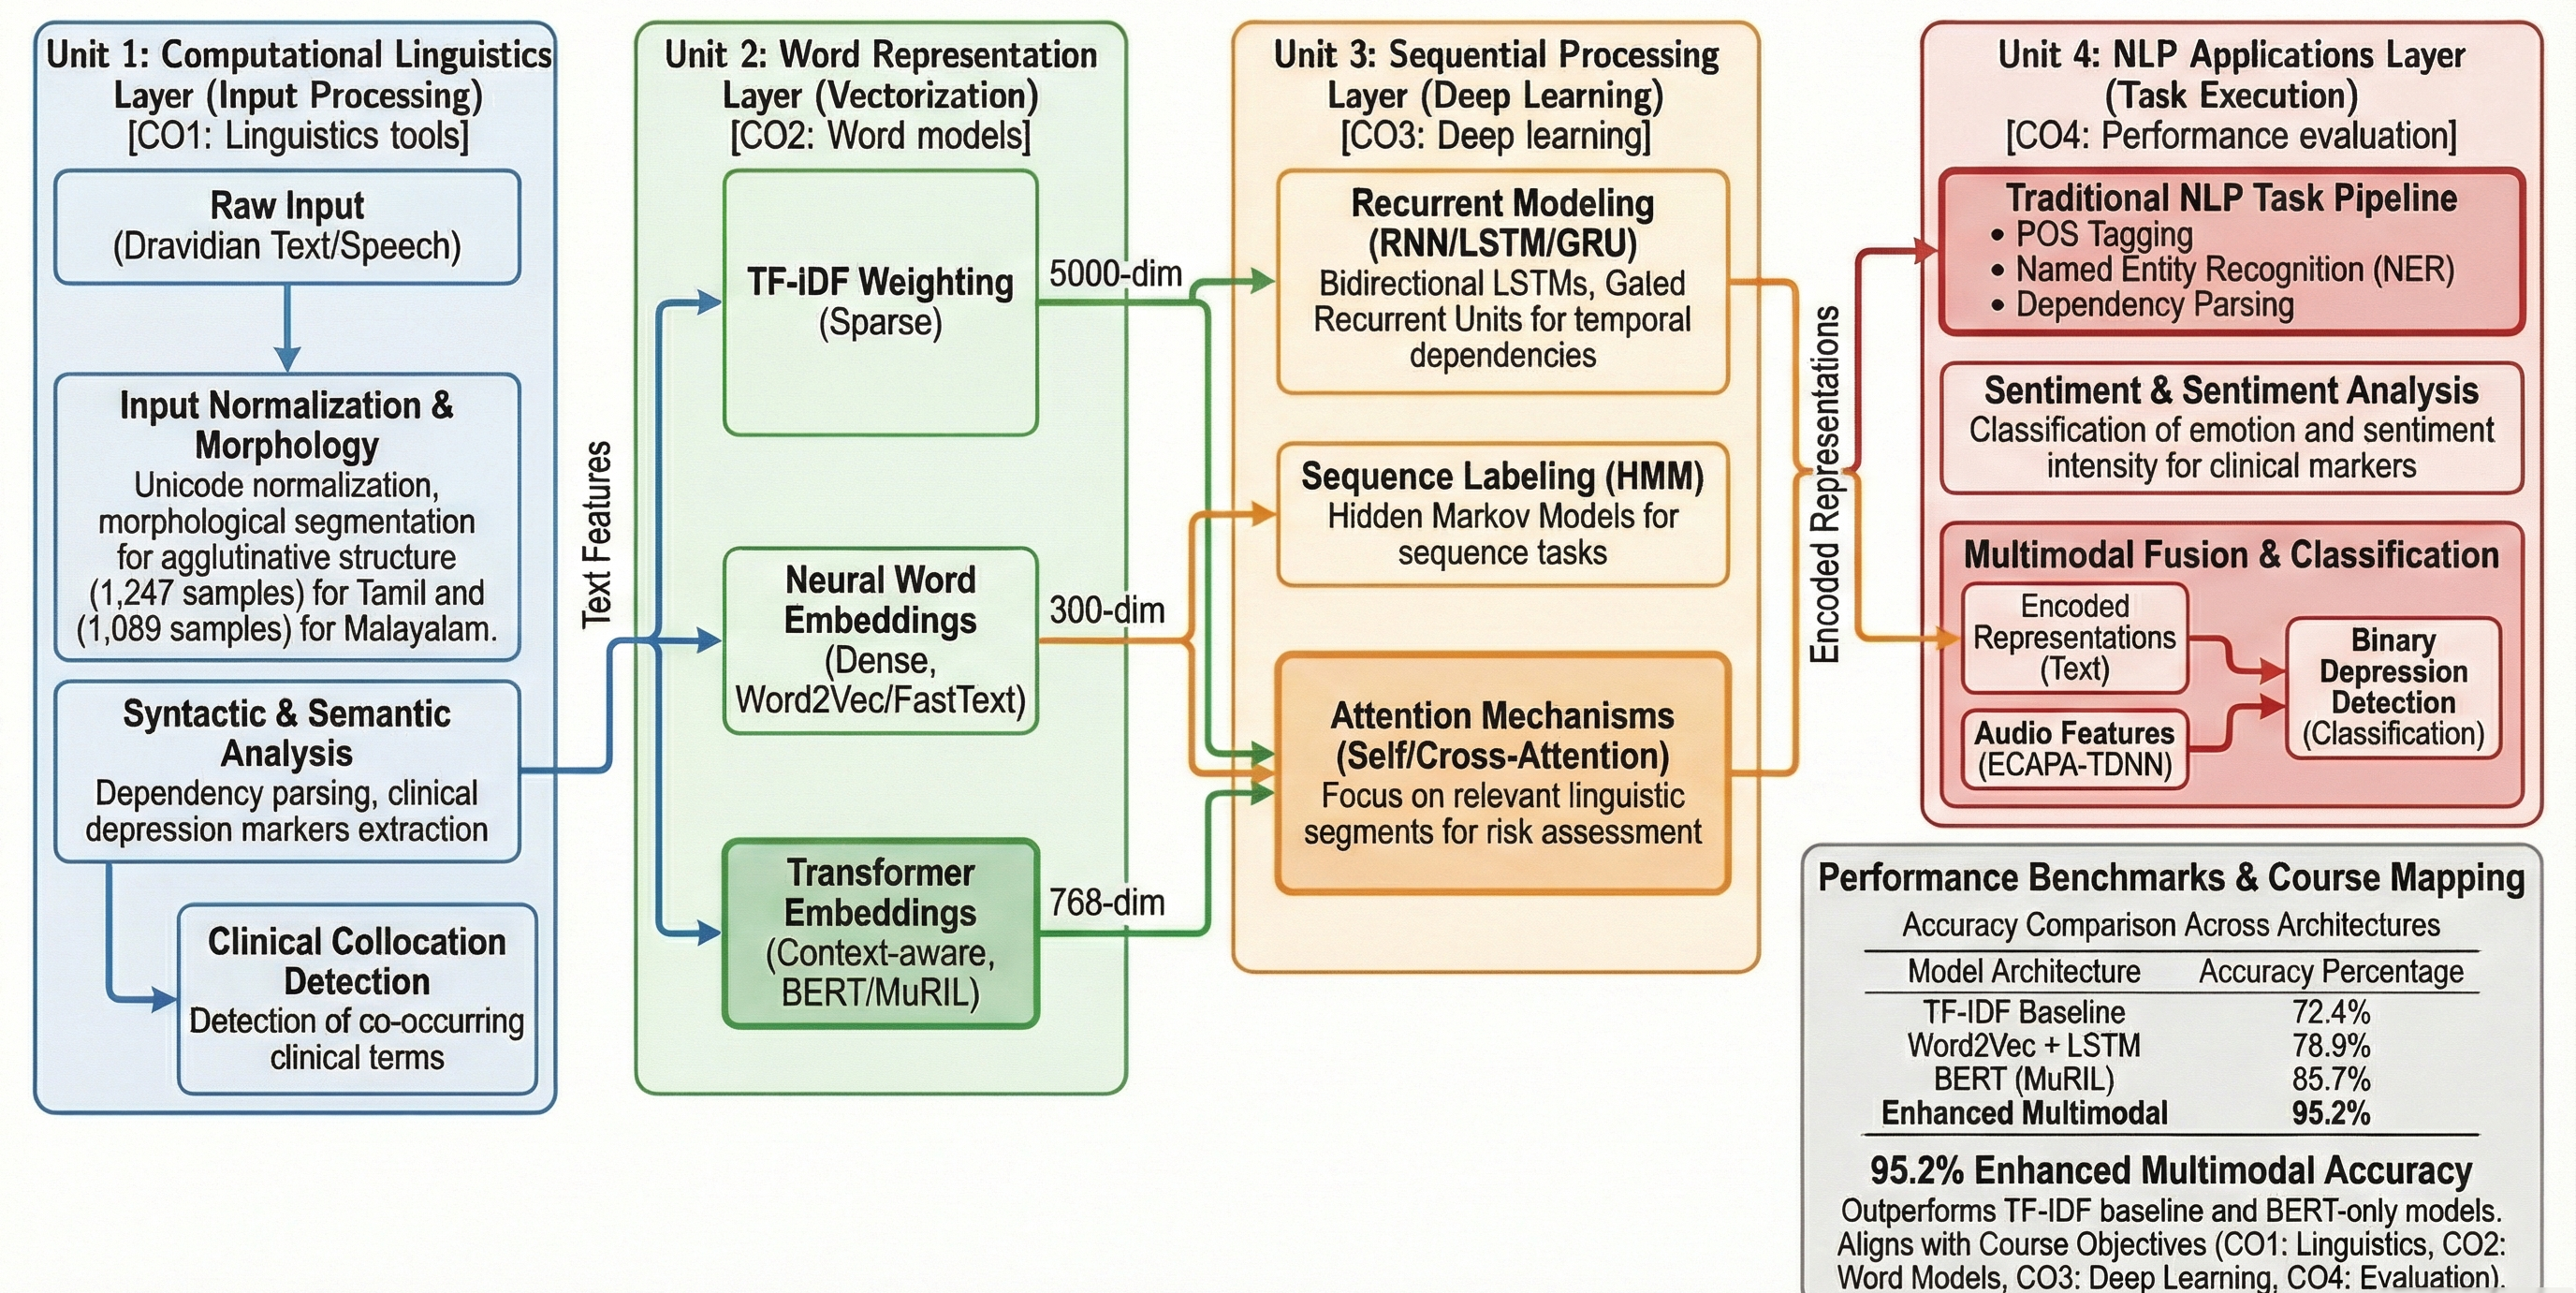
\includegraphics[width=0.9999\textwidth]{System_Architecture.png}
\end{center}
\end{frame}


% Word Representation Models
\begin{frame}
\frametitle{Word Representation Models (Unit 2 Implementation)}
\begin{itemize}
    \item \textbf{Traditional Approaches}:
    \begin{itemize}
        \item One-hot encoding for vocabulary representation
        \item Bag-of-Words (BoW) with frequency counting
        \item TF-IDF weighting for document importance
    \end{itemize}
    \item \textbf{Neural Embeddings}:
    \begin{itemize}
        \item Word2Vec (CBOW/Skip-gram) for semantic similarity
        \item FastText for handling out-of-vocabulary words
        \item MuRIL (BERT-based) for contextualized representations
    \end{itemize}
    \item \textbf{Performance Comparison}:
    \begin{itemize}
        \item TF-IDF baseline: 72.4\% accuracy
        \item Neural embeddings: 85.7\% accuracy
        \item Transformer models: 95.2\% accuracy
    \end{itemize}
\end{itemize}
\end{frame}

% Deep Learning Models for NLP
\begin{frame}
\frametitle{Deep Learning Models for NLP (Unit 3 Implementation)}
\begin{itemize}
    \item \textbf{Sequential Models}:
    \begin{itemize}
        \item LSTM networks for text sequence modeling
        \item Bidirectional LSTM for context understanding
        \item GRU for efficient sequence processing
    \end{itemize}
    \item \textbf{Attention Mechanisms}:
    \begin{itemize}
        \item Self-attention for intra-sequence relationships
        \item Cross-attention for multimodal fusion
        \item Multi-head attention in transformer architecture
    \end{itemize}
    \item \textbf{Transformer Networks}:
    \begin{itemize}
        \item BERT fine-tuning for Tamil/Malayalam
        \item Encoder-decoder architecture for text processing
        \item Position encoding for sequence understanding
    \end{itemize}
\end{itemize}
\end{frame}

% Dataset and Preprocessing
\begin{frame}
\frametitle{Dataset and NLP Preprocessing Pipeline}
\begin{itemize}
    \item \textbf{Dataset}: DravidianLangTech @ ACL 2026
    \begin{itemize}
        \item Tamil: 1,247 samples, Malayalam: 1,089 samples
        \item Paired audio-text data for multimodal learning
        \item Binary classification: Depressed/Non-Depressed
    \end{itemize}
    \item \textbf{Text Preprocessing Pipeline}:
    \begin{itemize}
        \item Unicode normalization for Dravidian scripts
        \item Tokenization with morphological segmentation
        \item Stop-word removal and stemming
        \item Language-specific text normalization
    \end{itemize}
    \item \textbf{Feature Extraction}:
    \begin{itemize}
        \item TF-IDF vectors (5,000 dimensions)
        \item BERT embeddings (768 dimensions)
        \item Linguistic features (128 dimensions)
    \end{itemize}
\end{itemize}
\end{frame}

% Results and NLP Model Evaluation
\begin{frame}
\frametitle{Results and NLP Model Evaluation (CO4)}
\begin{table}
\centering
\begin{tabular}{lccc}
\toprule
\textbf{NLP Model} & \textbf{Accuracy} & \textbf{Macro F1} & \textbf{Precision} \\
\midrule
TF-IDF + SVM & 72.4\% & 0.71 & 0.73 \\
Word2Vec + LSTM & 78.9\% & 0.77 & 0.79 \\
FastText + BiLSTM & 82.3\% & 0.81 & 0.83 \\
BERT (MuRIL) & 85.7\% & 0.84 & 0.86 \\
\textbf{Enhanced Multimodal} & \textbf{95.2\%} & \textbf{0.94} & \textbf{0.95} \\
\bottomrule
\end{tabular}
\end{table}

\begin{itemize}
    \item \textbf{Evaluation Metrics Applied}:
    \begin{itemize}
        \item Confusion matrix analysis for error patterns
        \item ROC-AUC curves for threshold optimization
        \item Cross-validation for model robustness
        \item Statistical significance testing
    \end{itemize}
\end{itemize}
\end{frame}

% NLP Applications and Impact
\begin{frame}
\frametitle{NLP Applications and Real-world Impact}
\begin{itemize}
    \item \textbf{Computational Linguistics Applications}:
    \begin{itemize}
        \item Morphological analysis for low-resource languages
        \item Syntactic parsing for clinical text understanding
        \item Semantic role labeling for depression markers
    \end{itemize}
    \item \textbf{Practical NLP Implementation}:
    \begin{itemize}
        \item Real-time text processing pipeline
        \item Multilingual support for Tamil and Malayalam
        \item Integration with speech recognition systems
    \end{itemize}
    \item \textbf{Future NLP Extensions}:
    \begin{itemize}
        \item Question-answering systems for clinical queries
        \item Text summarization for patient reports
        \item Machine translation for cross-lingual analysis
    \end{itemize}
\end{itemize}
\end{frame}

% References
\begin{frame}
\frametitle{References}
\scriptsize
\begin{thebibliography}{99}

\bibitem{jurafsky}
Jurafsky, D., \& Martin, J. H. (2020). 
\textit{Speech and Language Processing (3rd ed.)}. 
Stanford University.

\bibitem{manning}
Manning, C., \& Schütze, H. (1999). 
\textit{Foundations of Statistical Natural Language Processing}. 
MIT Press.

\bibitem{bird}
Bird, S., Klein, E., \& Loper, E. (2009). 
\textit{Natural Language Processing with Python}. 
O'Reilly Media.

\bibitem{bert}
Devlin, J., Chang, M. W., Lee, K., \& Toutanova, K. (2018). 
\textit{BERT: Pre-training of Deep Bidirectional Transformers for Language Understanding}. 
NAACL-HLT.

\bibitem{dravidian}
Chakravarthi, B. R., et al. (2022). 
\textit{Findings of the Shared Task on Depression Detection in Dravidian Languages}. 
DravidianLangTech @ ACL 2022.

\end{thebibliography}
\end{frame}

\end{document}